\chapter{Énoncé du problème}
\label{ennonce}
\lhead{Chapitre 2 - Énoncé du problème}
La gestion des programme de cours n'est pas une chose aisée. La situation est complexe essentiellement pour deux raisons.
\begin{enumerate}
\item La \textit{commission INFO} s'occupe d'un nombre assez élevé de programmes;
\item il existe des contraintes de différentes sortes qui restreignent les étudiants dans les choix qu'ils peuvent faire lorsqu'ils configurent leur programme de cour;
\item les programmes évoluent souvent.
\end{enumerate}

Ces trois points vont être présentés en détail dans les sections qui suivent. 


\section{Programmes proposés}
La liste des programmes proposés par la \textit{commission INFO} est la suivante:


\textbf{Bachelier en sciences informatiques - SINF1BA} \cite{SINF1BA} - C'est un programme de 180 crédits. Comme dans tout programme de bachelier à l'UCL, l'étudiant est amené à devoir choisir une mineure dans ce programme. Par exemple, une mineure intitulée \textit{Approfondissement en sciences informatiques} est disponible pour les étudiants qui suivent ce programme. La durée normale de ce programme de bachelier est de trois ans. 

\textbf{Bachelier en sciences de l'ingénieur, orientation ingénieur civil - FSA1BA (Majeure ou Mineure en informatique)} - \cite{FSA1BA}. Ici il n'est pas question du programme FSA1BA dans son entièreté mais de la majeure ou mineure que l'étudiant en sciences de l'ingénieur est amené à choisir lorsqu'il suit ce programme.

\textbf{Master [120] en sciences informatiques - SINF2M} \cite{SINF2M} - Ce programme de 120 crédits est destiné aux étudiants en provenance du programme \textit{SINF1BA}. Il comporte un module obligatoire (le tronc commun) et la possibilité de choisir un ou plusieurs modules optionnels (Génie logiciel, systèmes de programmation, intelligence artificielle, réseaux et sécurité). La charge du travail de fin d'étude est de 28 crédits. La durée normale de ce programme de master est de deux ans.

\textbf{Master [60] en sciences informatiques - SINF2M1} \cite{SINF2M1} - Ce programme alternatif de 60 crédits est destiné aux étudiants en provenance du programme \textit{SINF1BA}. Il comporte un module obligatoire (le tronc commun) et la possibilité de choisir quelques cours au choix mais pas d'options. La charge du travail de fin d'étude est plus petite que celle de son homologue  \textit{SINF2M}: 18 crédits. La durée normale de ce programme de master est d'un an. 

\textbf{Master [120] : ingénieur civil en informatique - INFO2M} \cite{INFO2M} - Ce programme est destiné aux étudiants en provenance du programme \textit{FSA1BA} ayant suivi soit la mineure soit la majeure en informatique. Comme dans le master \textit{SINF2M}, il comporte un module obligatoire (le tronc commun) ainsi que la possibilité de choisir un ou plusieurs modules optionnels (Génie logiciel, systèmes de programmation, intelligence artificielle, réseaux et sécurité). La charge du travail de fin d'étude est de 28 crédits. La durée de ce programme de master est de deux ans.  

\textbf{Année d'études préparatoire au master en sciences informatiques - SINF1PM} \cite{SINF1PM} - Ce programme est destiné aux étudiants en provenance de Hautes écoles d'informatique. Il permet d'accéder aux programmes \textit{SINF2M} et \textit{SINF2M1}. C'est un programme \textit{à la carte} qui dépend du \textit{background} de l'étudiant (Dans la plupart des cas, c'est un programme standard qui est proposé). Les cours sont choisis parmi ceux proposés dans le programme \textit{SINF1BA}. Ce programme affiche entre 46 et 60 crédits. La durée normale de ce programme est d'un an.  
 

Outre ces programmes, \textit{la commission INFO} doit s'occuper du cas des étudiants en programme d'échange. La principale difficulté, que cela soit un étudiant immigrant ou émigrant, est de trouver des équivalences entre les cours suivis dans l'université d'origine et ceux proposés à l'UCL ou l'inverse. 

De plus, les intersections entre ces cours sont nombreuses. Beaucoup de cours sont disponibles pour une partie voir la totalité des programmes cités ci-dessus.  
\clearpage
\section{Contraintes}
\label{contraintes_intro}

Les contraintes sont un point important du problème. En plus d'être nombreuses et diversifiées, elles requièrent beaucoup de travail au niveau de leur vérification du coté de \textit{la commission INFO}. En outre, elles sont difficiles à exprimer (et vérifier) avec les moyens (formulaire excel, présentation en début d'année, portail du département) mis à la disposition de l'équipe. La conséquence directe de ceci est qu'il est difficile pour les étudiants de comprendre le pourquoi du comment de ces contraintes. Ils n'en tiennent donc pas compte à 100\% lorsqu'ils construisent leur programme de cours.

Voici une liste qui en présente brièvement les différentes sortes que l'on peut rencontrer.
\begin{enumerate}
\item \textbf{Dépendances entre les différents cours} - Ces contraintes  sont de deux types :
	\begin{enumerate}
	\item Les prérequis : Les prérequis d'un cours sont les cours qu'il faut avoir réussis (dans des années académiques antérieures) afin de pouvoir suivre ce cours 
	\item Les corequis : Les corequis d'un cours sont les cours qu'il faut avoir suivis \textbf{au plus tard} durant la même année académique que ce cours.
	\end{enumerate} 

L'image~\ref{fig:cour_dep} illustre ce type de contrainte. On peut voir que le cours \textit{INGI2365} a pour prérequis le cours \textit{SINF1121} et pour corequis le cours \textit{INGI2261}. Il est donc nécessaire d'avoir \textbf{validé} \textit{SINF1121} ainsi que de suivre (au plus tard) \textbf{durant la même période} le cours \textit{INGI2261} (s'il n'a pas été suivi précédemment) pour avoir accès à \textit{INGI2365}. Ces deux contraintes sont directionnelles! le cours \textit{SINF1121} n'a pas pour corequis le cours \textit{INGI2365}, de même que le cours \textit{INGI2261} n'a pas pour prérequis le cours \textit{INGI2365}. 

Notez que l'arrête qui relie le cours \textit{SINF1121} au cours \textit{INGI2365} est interprétée comme directionnelle dans le logiciel. 

\begin{figure}[H]
\centering
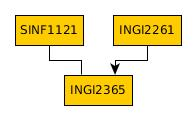
\includegraphics{dependancies_ex}
\caption{Dépendances du cours INGI2261}
\label{fig:cour_dep}
\end{figure}

\item \textbf{Contraintes induites par les programmes} - Ce sont les différents cours ou ensembles de cours qu'il est obligatoire de suivre avant de valider un programme. En master, il y a, par exemple, le module intitulé \textit{Tronc Commun} qu'il est obligatoire de suivre, ainsi que le mémoire. Certains modules optionnels, comme les options de master, sont constitués de sous-modules dont il est obligatoire de suivre la totalité des cours qu'ils contiennent. 

\item \textbf{Contraintes temporelles} - Ce sont les contraintes les plus basiques. Elles représentent la période de temps durant laquelle il est possible de suivre le cours en question. Initialement, elles sont exprimées en terme de semestre. Pour des raisons variables, comme un professeur qui part à la retraite, ou qui prend une année sabbatique, elles peuvent très bien s'exprimer en terme d'années académiques. Un autre exemple sont les cours bisannuels qui sont des cours se donnant une fois tous les deux ans. 

\item \textbf{Contraintes sur les propriétés} - Ces contraintes portent sur les propriétés des cours, programmes ou modules. Principalement, elles portent sur les crédits minimum et maximum d'un programme ou d'un module.

\end{enumerate}


\section{Conclusion}
L'objectif est de développer une application pour que la charge des différents problèmes présentés plus haut (la gestion des contraintes, le nombre des programmes proposés et leur complexité) soit à la charge d'une machine. L'idée est de pouvoir:
\begin{itemize}
\item importer et mettre à jour les données relatives aux catalogues de cours;
\item permettre aux étudiants de conserver un historique des cours et programmes qu'ils ont déjà suivis au cours des années précédentes (et des catalogues d'où proviennent ces cours);
\item visualiser ces données, que l'on soit étudiant ou membre de la commission de programme;
\item effectuer une vérification immédiate de la validité des programmes de cours créés par les étudiants;


\item permettre à la commission de communiquer avec les étudiants via l'application, pour par exemple attirer l'attention de l'étudiant sur une partie de son programme qui ne semble pas cohérente, ou dans l'autre sens, demander ou donner des explications à la commission sur certains points;
\item porter l'application aisément en production (via le \textit{"cloud"} par exemple). 
\end{itemize}

De manière plus générale, le but de ce mémoire est de développer une application conviviale, maintenable et évolutive afin qu'elle puisse être utilisée par les étudiants et la commission de programme. 

Ce mémoire sera typiquement un projet que pourrait rencontrer un informaticien dans la vie active, où la \textit{commission INFO} joue le rôle de client, et le promoteur celui de chef de projet. 